\chapter{\label{sec:filtros} Experimento I - Filtros}
\begin{figure}[hbt]
\begin{center}
\begin{circuitikz}[scale=1]
		\draw
			(0,0) node[ground] {}
			to [sinusoidal voltage source, o-o, l=$\epsilon(t)$] ++(0,2)
			to [generic, o-o, l=$Z_g$] ++(2,0)
			to [generic, o-o, l=$Z_1$] ++(2,0)
			(4,2) to [short,o-o] ++(1,0)
			(4,2) to [generic, o-o, l=$Z_2$] ++(0,-2)
			node[ground] {}
			;
		%Description of subparts
		\draw [decorate,decoration={brace,amplitude=8pt},
					xshift=0pt, yshift=0pt]
					(2,-1) -- (-0.5,-1)
					node[black,midway,yshift=-20pt]
						{Gerador AC};
		\draw [decorate,decoration={brace,amplitude=8pt},
					xshift=0pt, yshift=0pt]
					(5,-1) -- (2.1,-1)
					node[black,right,yshift=-20pt]
						{Circuito de duas portas};	
	\end{circuitikz}
  \caption{Generic two-port circuit setup. $Z_g$ represents the internal impedance of the AC generators, $Z_1,Z_2$ are any generic linear circuit components. The arrows $V_1$ and $V_2$ indicate where we connect  oscilloscope channels to the circuit. }
  \end{center}
  \label{fig:generic_two_port}
\end{figure}
%----------------------------------
%-------OBJETIVOS------------------
%----------------------------------
\subsection{Objetivos}
Entender o papel ...
\subsection{Introdu��o}
Introduction goes here...
\subsubsection{Diodo demodulador ou detector}
% \begin{wrapfigure}{r}{0.5\textwidth}
%  \vspace{-20pt}
%  \begin{center}
%    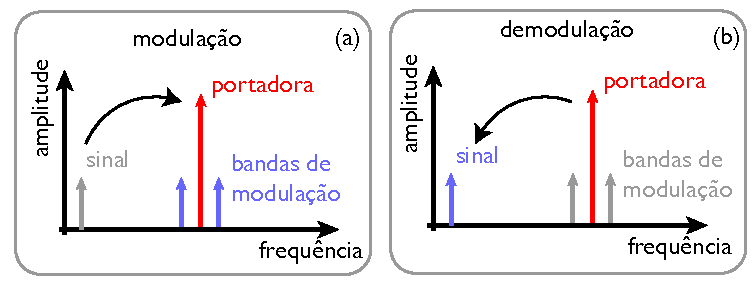
\includegraphics[width=0.5\textwidth]{mod_e_demod}
%  \end{center}
%   \vspace{-20pt}
%  \caption{Princ�pio de modula��o de demodula��o de um sinal.}
%\end{wrapfigure}
%----------------------------------
%-------PREPARA��O-----------------
%----------------------------------
\subsection{Prepara��o}
\begin{enumerate}
\item Calcule a fun��o... 
\end{enumerate}
%----------------------------------
%-------MATERIAL-----------------
%----------------------------------

%----------------------------------
%----------Roteiro-----------------
%----------------------------------
\subsection{Roteiro A - Circuito RC}
\begin{figure}
\centering
\subfigure[Circuito RC com tens�o de sa�da medida no capacitor, $V_2=\frac{1}{j\omega C}i$]{
\tpnc{resistor}{R}{capacitor}{C}}
\subfigure[Circuito RC com tens�o de sa�da medida no resistor, $V_2=R i$]{
\tpnc{capacitor}{C}{resistor}{R}}
\end{figure}


\subsubsection*{Material}
\begin{itemize}
\item Diodo de  sil�cio.
\end{itemize}
\subsubsection*{Caracteriza��o do circuito LC}
\subsection{Roteiro B - Circuito RLC}
Nesta etapa desejamos estudar experimentalmente o fen�meno de resson�ncia em circuitos RLC. Iremos determinar a resposta em frequ�ncia deste circuito (amplitude e fase) e investigar suas principais caracter�sticas, frequ�ncia de resson�ncia, largura de banda e pot�ncia dissipada.
\begin{figure}[hb]
\subfigure[ ]{
\begin{circuitikz}[scale=.8]
		\node (Xi) at (0.7,0.7) {$V_1$};
		\node (Xf) at (5.7,0.7) {$V_2$};
		\draw [semithick,->] (Xi) -- (0.1,0.1);
		\draw [semithick,->] (Xf) -- (5.1,0.1);
		\draw	to [inductor, o-o, l_=L] ++(2,0)
				to [capacitor, o-o, l_=C] ++(2,0)
				(4,0) to [short,o-o] ++(1,0)
				(4,0) to [resistor, o-o, l=R] ++(0,-2)
				node[ground] {};
	\end{circuitikz}}
\subfigure[ ]{
\begin{circuitikz}[scale=.8]
		\node (Xi) at (0.7,0.7) {$V_1$};
		\node (Xf) at (5.7,0.7) {$V_2$};
		\draw [semithick,->] (Xi) -- (0.1,0.1);
		\draw [semithick,->] (Xf) -- (5.1,0.1);
		\draw	to [resistor, o-o, l_=R] ++(2,0)
				to [capacitor, o-o, l_=C] ++(2,0)
				(4,0) to [short,o-o] ++(1,0)
				(4,0) to [inductor, o-o, l=L] ++(0,-2)
				node[ground] {};
	\end{circuitikz}}
\subfigure[ ]{
\begin{circuitikz}[scale=.8]
		\node (Xi) at (0.7,0.7) {$V_1$};
		\node (Xf) at (5.7,0.7) {$V_2$};
		\draw [semithick,->] (Xi) -- (0.1,0.1);
		\draw [semithick,->] (Xf) -- (5.1,0.1);
		\draw	to [inductor, o-o, l_=L] ++(2,0)
				to [resistor, o-o, l_=R] ++(2,0)
				(4,0) to [short,o-o] ++(1,0)
				(4,0) to [capacitor, o-o, l=C] ++(0,-2)
				node[ground] {};
	\end{circuitikz}}
	\caption{\textbf{Diferentes configura��es de um filtro RLC}. }
\end{figure}
\subsubsection*{Caracteriza��o da curva IV do diodo}
%----------------------------------
%----------Relatorio-----------------
%----------------------------------
\subsection{Relat�rio}

